\documentclass[11pt]{article}

% Template-agnostic paper: swap to your conference class as needed.
\usepackage[margin=1in]{geometry}
\usepackage{times}
\usepackage{microtype}
\usepackage{graphicx}
\usepackage{booktabs}
\usepackage{amsmath, amssymb}
\usepackage{enumitem}
\usepackage{hyperref}
\usepackage{url}
\usepackage{xspace}
\usepackage{placeins} % \FloatBarrier

\newcommand{\github}{\raisebox{-1.5pt}{
\includegraphics[height=1.05em]{figures/github.png}}\xspace}

\setlength{\parindent}{0pt}

\title{MIRAGE-V: A Taxonomy-Driven Benchmark for Physics Verification in Videos}

\date{}

% Auto-generated after you run experiments.
% Auto-generated from overall.csv
\newcommand{\NumExamples}{1000}
\newcommand{\NumModules}{10}
\newcommand{\FramesPerVideo}{8}

% Best-performing models on aggregate metrics
\newcommand{\BestAccModel}{GPT-5.2}
\newcommand{\BestAcc}{61.0}

\newcommand{\BestPairModel}{Gemini-2.5-Flash}
\newcommand{\BestPairAcc}{27.4}


\begin{document}
\maketitle

\begin{abstract}
Video reasoning models increasingly act as general-purpose ``world models'' for downstream tasks such as robotics, simulation validation, and safety monitoring, yet existing video benchmarks often conflate temporal reasoning with static shortcuts, provide limited diagnostic structure, or emphasize generative plausibility rather than falsifiable physics checking.
We introduce \textbf{MIRAGE-V}, a taxonomy-driven benchmark for \emph{physics verification in videos} built from \emph{minimal-change paired clips} that differ by a single controlled intervention aligned to a specific failure category (e.g., temporal aliasing, occlusion-induced identity drift, latent physical property inference, and conservation-law violations).
Each example is annotated with a \emph{critical time window}, enabling sampling-robust evaluation and optional temporal localization.
We release an open-source generator for scalable pair creation, a unified evaluation harness supporting both open-weight and API-accessible models, and standardized analysis protocols with shortcut audits (text-only, single-frame, shuffled frames, and sparse-vs-dense sampling).
Across a \NumExamples-example evaluation spanning \NumModules\ taxonomy modules with \FramesPerVideo uniformly sampled frames per video, the best-performing model achieves \BestAcc\% accuracy but only \BestPairAcc\% pair accuracy, revealing that even frontier models frequently fail to discriminate minimally different clips and to reliably detect subtle physical inconsistencies.
These findings highlight a persistent gap between apparent video understanding and true physics checking, with important implications for deploying video reasoning systems in safety-critical and decision-making settings.

\end{abstract}

\section{Introduction}
Frontier video-language models can answer a wide range of questions about complex scenes, but they frequently fail on \emph{physics checking}: detecting subtle inconsistencies such as discontinuous motion, identity swaps under occlusion, or uncaused changes in energy or momentum.
These failure modes matter in high-stakes settings (robotics, surveillance, simulation validation), where a system must not only describe what it sees but also flag implausible or impossible events.

Existing video understanding benchmarks provide broad coverage, but many tasks can be solved with weak temporal reasoning (e.g., static frames, language priors, or dataset artifacts), which reduces diagnostic value.
Conversely, physics-focused datasets often emphasize \emph{prediction} (``what happens next?'') rather than \emph{verification} (``did an impossible event occur?'') or they focus on a narrow set of physical principles.
Recent work on evaluating video \emph{generation} models as world models highlights the importance of physics adherence, but typically evaluates \emph{generated} videos and uses human preference labels \cite{li2025worldmodelbench}.
Our focus is complementary: we evaluate \emph{video reasoning} models on whether they can \emph{detect} minimal physical inconsistencies in observed clips.

\paragraph{Benchmark design principles.}
MIRAGE-V is built around three principles:
(1) \textbf{Minimal-change pairs} --- each datapoint is part of an $A/B$ pair that shares context but differs by a single intervention, enabling causal attribution and the \emph{pair accuracy} metric;
(2) \textbf{Taxonomy-driven failures} --- interventions are mapped to a small set of interpretable modules (taxonomy categories) covering temporal, occlusion, latent-parameter, invariant, and causal phenomena;
(3) \textbf{Sampling-robust evaluation} --- each example provides a critical window when decisive evidence occurs, supporting both sparse and dense sampling protocols.

\paragraph{Contributions.}
We contribute:
(i) \textbf{MIRAGE-V}, a benchmark suite of minimal-change video pairs with taxonomy labels and critical-window annotations;
(ii) an \textbf{open-source generator} that produces scalable synthetic clips and optional real-video edits aligned to the taxonomy;
(iii) a \textbf{unified evaluation harness} for open-weight and API-based models with standardized prompting, metrics, and shortcut audits;
(iv) an empirical baseline on three representative models demonstrating that physics checking remains challenging, especially under sparse frame sampling.

\section{Related Work}
\paragraph{Video-language understanding benchmarks.}
A growing body of work evaluates multi-modal models on video question answering and temporal reasoning, including TVQA \cite{lei2018tvqa}, NExT-QA \cite{xiao2021nextqa}, EgoSchema \cite{mangalam2023egoschema}, MVBench \cite{li2023mvbench}, and Video-MME \cite{fu2024videomme}.
These benchmarks provide broad coverage across domains and temporal scales, but are not designed around \emph{minimal physical interventions} and often permit shortcuts (e.g., static cues or language priors) that reduce their sensitivity to subtle physics violations.

\paragraph{Physics and intuitive-physics datasets.}
Synthetic physics datasets such as CLEVRER \cite{yi2019clevrer} probe causal, predictive, and counterfactual reasoning about object interactions.
IntPhys \cite{riochet2018intphys} and IntPhys~2 \cite{bordes2025intphys2} evaluate intuitive physics via violation-of-expectation tests.
Physion++ \cite{tung2023physionpp} emphasizes inference of \emph{latent} physical properties (mass, friction, elasticity) from observed dynamics.
MIRAGE-V is complementary: we focus on \emph{verification} of minimal-change paired clips and provide taxonomy labels plus a critical window to audit sampling sensitivity.

\paragraph{Benchmarks for ``world models'' and generative video.}
WorldModelBench \cite{li2025worldmodelbench} evaluates video generation models along instruction following and physics adherence, leveraging large-scale human preference labels.
While it targets generated videos and preference judgments, MIRAGE-V targets \emph{observed} clips and asks models to answer falsifiable questions about specific physical violations, with paired construction enabling rigorous discrimination metrics.

\paragraph{Taxonomy-driven evaluation.}
RF100-VL \cite{robicheaux2025roboflow100vl} illustrates how taxonomy and dataset composition can expose out-of-distribution weaknesses in vision-language models.
MIRAGE-V applies a similar philosophy to video physics checking: a compact, interpretable taxonomy and controlled interventions provide a diagnostic view of model failure modes.

\section{MIRAGE-V Benchmark}
\subsection{Taxonomy modules}
MIRAGE-V organizes physics-checking failures into \NumModules\ taxonomy modules: \textbf{TR-ALI} (temporal aliasing), \textbf{TR-ORDER} (temporal order), \textbf{TM-ID} (tracking/identity), \textbf{P-OCC} (hidden interactions), \textbf{R-COUNT} (relational counting), \textbf{PH-LATENT-MASS} and \textbf{PH-LATENT-FRICTION} (latent properties), \textbf{PH-INVAR-ENERGY} (invariants), \textbf{C-CHAIN} (causal chains), and \textbf{PH-COUNTER} (counterfactual).

\subsection{Minimal-change paired construction}
Each pair shares the same context but differs by a single intervention---either \emph{parameter edits} (swap mass/friction, add/remove obstacle) or \emph{state edits} (micro-teleportation, velocity boosts). Paired construction enables \emph{pair accuracy} (both $A$ and $B$ correct) and causal attribution.

\subsection{Schema and metrics}
Each example contains \texttt{pair\_id}, \texttt{pair\_role}, \texttt{prompt}, \texttt{answer\_index}, \texttt{video\_path}, \texttt{module}, and \texttt{critical\_window}. We report \textbf{accuracy} on individual examples, \textbf{pair accuracy} on minimal-change pairs, and \textbf{module breakdowns} for diagnostics.

\section{Experiments}
This section reports baseline results on three representative models and illustrates how MIRAGE-V exposes taxonomy-specific weaknesses.
All numbers in this section are computed from the released evaluation harness outputs (CSV summaries and per-example predictions).

\subsection{Setup}
We evaluate a MIRAGE-V suite of \NumExamples examples grouped into \NumModules modules (100 examples / 50 minimal pairs per module).
To enable apples-to-apples comparison across models with different native video interfaces, we use a \textbf{frame-based protocol}: each video is decoded into \textbf{\FramesPerVideo} uniformly sampled frames, and all models are prompted with the same sampled frames and a yes/no question.

\subsection{Models}
We evaluate:
\begin{itemize}[leftmargin=*]
  \item \textbf{GPT-5.2} (OpenAI API, frame inputs).
  \item \textbf{Gemini-2.5-Flash} (Gemini API, evaluated on the same sampled frames).
  \item \textbf{Qwen2.5-VL-7B} (open-weight, local inference via Hugging Face Transformers).
\end{itemize}
All models are instructed to answer \texttt{YES} or \texttt{NO} only (no explanation) to reduce parsing ambiguity.

\subsection{Aggregate performance}
Table~\ref{tab:overall} reports overall accuracy and pair accuracy.
GPT-5.2 achieves the highest individual-example accuracy (\BestAcc\%), while Gemini-2.5-Flash achieves the highest pair accuracy (\BestPairAcc\%).
However, pair accuracy remains below 28\% for all models, indicating that even when models answer single examples moderately well, they often fail to \emph{discriminate} minimally different clips.

\begin{table}[t]
  \centering
  \small
  \caption{Overall results on \NumExamples examples (\FramesPerVideo uniform frames per video). We bold the best score in each column.}
  \label{tab:overall}
  % Auto-generated from overall.csv
\begin{tabular}{lrrrr}
\toprule
Model & $N$ & Acc. (\%) & Pair Acc. (\%) \\
\midrule
GPT-5.2 & 1000 & \textbf{61.0} & 27.2 \\
Gemini-2.5-Flash & 1000 & 57.0 & \textbf{27.4} \\
Qwen2.5-VL-7B & 1000 & 53.5 & 20.8 \\
\bottomrule
\end{tabular}

\end{table}

\subsection{Accuracy by taxonomy module}
Figure~\ref{fig:by-module-accuracy} and Table~\ref{tab:by-module-accuracy} break down accuracy by taxonomy module.
We observe three consistent patterns:

\paragraph{(i) Near-chance accuracy hides shortcut behavior.}
Several modules cluster near 50\% accuracy (e.g., C-CHAIN, P-OCC, TM-ID, PH-INVAR-ENERGY).
Because MIRAGE-V pairs flip the correct answer between $A$ and $B$ by construction, a model that defaults to one answer can achieve $\approx$50\% accuracy while failing to detect the intervention.

\paragraph{(ii) Coarse temporal aggregation is easier than fine-grained physics checking.}
Counting (R-COUNT) is comparatively easy for all models, with near-perfect accuracy for GPT-5.2 and Qwen2.5-VL-7B.
Event ordering (TR-ORDER) is also relatively easier for Gemini and Qwen, while GPT-5.2 is near chance on this module under sparse sampling.

\paragraph{(iii) Latent-property inference remains challenging.}
Inferring mass and friction from dynamics (PH-LATENT-MASS / PH-LATENT-FRICTION) exposes clear gaps across models.
In particular, PH-LATENT-FRICTION is the hardest module on average, and Qwen2.5-VL-7B fails completely on this module in this evaluation protocol.

\begin{figure}[t]
  \centering
  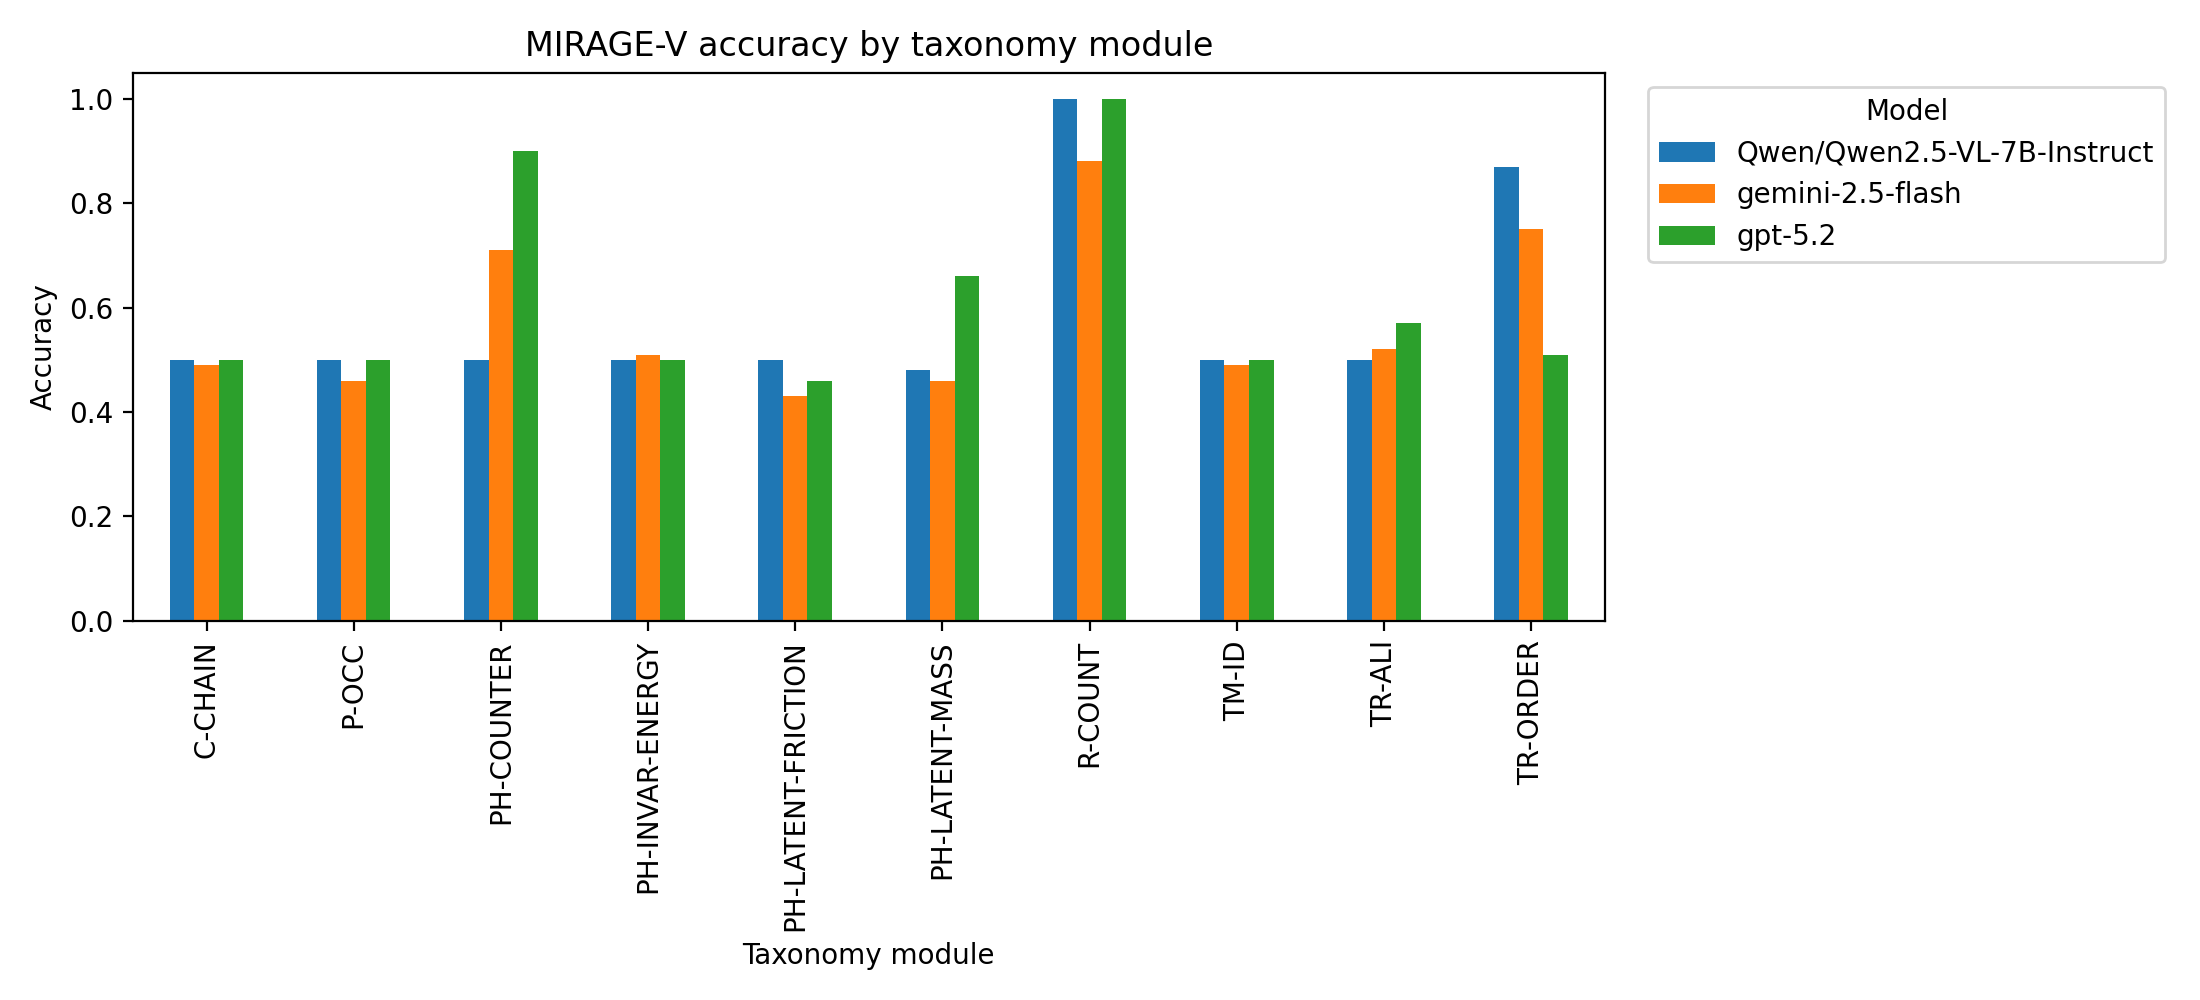
\includegraphics[width=\linewidth]{figures/by_module_accuracy.png}
  \caption{Accuracy by MIRAGE-V taxonomy module for three representative models. All models are evaluated with \FramesPerVideo uniformly sampled frames per video.}
  \label{fig:by-module-accuracy}
\end{figure}

\begin{table}[t]
  \centering
  \small
  \caption{Per-module accuracy (\%, higher is better). Each module contains 100 examples (50 minimal-change pairs).}
  \label{tab:by-module-accuracy}
  % Auto-generated from by_module.csv
\begin{tabular}{lrrr}
\toprule
Module & Qwen2.5-VL-7B & Gemini-2.5-Flash & GPT-5.2 \\
\midrule
C-CHAIN & \textbf{50.0} & 49.0 & \textbf{50.0} \\
P-OCC & \textbf{50.0} & 46.0 & \textbf{50.0} \\
PH-COUNTER & 50.0 & 71.0 & \textbf{90.0} \\
PH-INVAR-ENERGY & 50.0 & \textbf{51.0} & 50.0 \\
PH-LATENT-FRICTION & 0.0 & 43.0 & \textbf{46.0} \\
PH-LATENT-MASS & 48.0 & 46.0 & \textbf{66.0} \\
R-COUNT & \textbf{100.0} & 88.0 & \textbf{100.0} \\
TM-ID & \textbf{50.0} & 49.0 & \textbf{50.0} \\
TR-ALI & 50.0 & 52.0 & \textbf{57.0} \\
TR-ORDER & \textbf{87.0} & 75.0 & 51.0 \\
\bottomrule
\end{tabular}

\end{table}

\subsection{Pair accuracy by taxonomy module}
Pair accuracy is a stricter metric: a pair is correct only if the model answers \emph{both} minimally different videos correctly.
Figure~\ref{fig:by-module-pair-accuracy} and Table~\ref{tab:by-module-pair-accuracy} show that pair accuracy is substantially lower than accuracy for most modules.

\paragraph{Discrimination failures.}
Modules with $\approx$50\% accuracy but near-zero pair accuracy (e.g., C-CHAIN, TM-ID, P-OCC, PH-INVAR-ENERGY for some models) indicate that the model often gives the same answer for both $A$ and $B$ and does not detect the causal intervention.

\paragraph{Sampling sensitivity.}
TR-ALI (micro-teleportation) exhibits low pair accuracy for all models, consistent with sparse sampling missing brief violations.
This motivates MIRAGE-V's critical-window annotations and sparse-vs-dense reporting.

\begin{figure}[t]
  \centering
  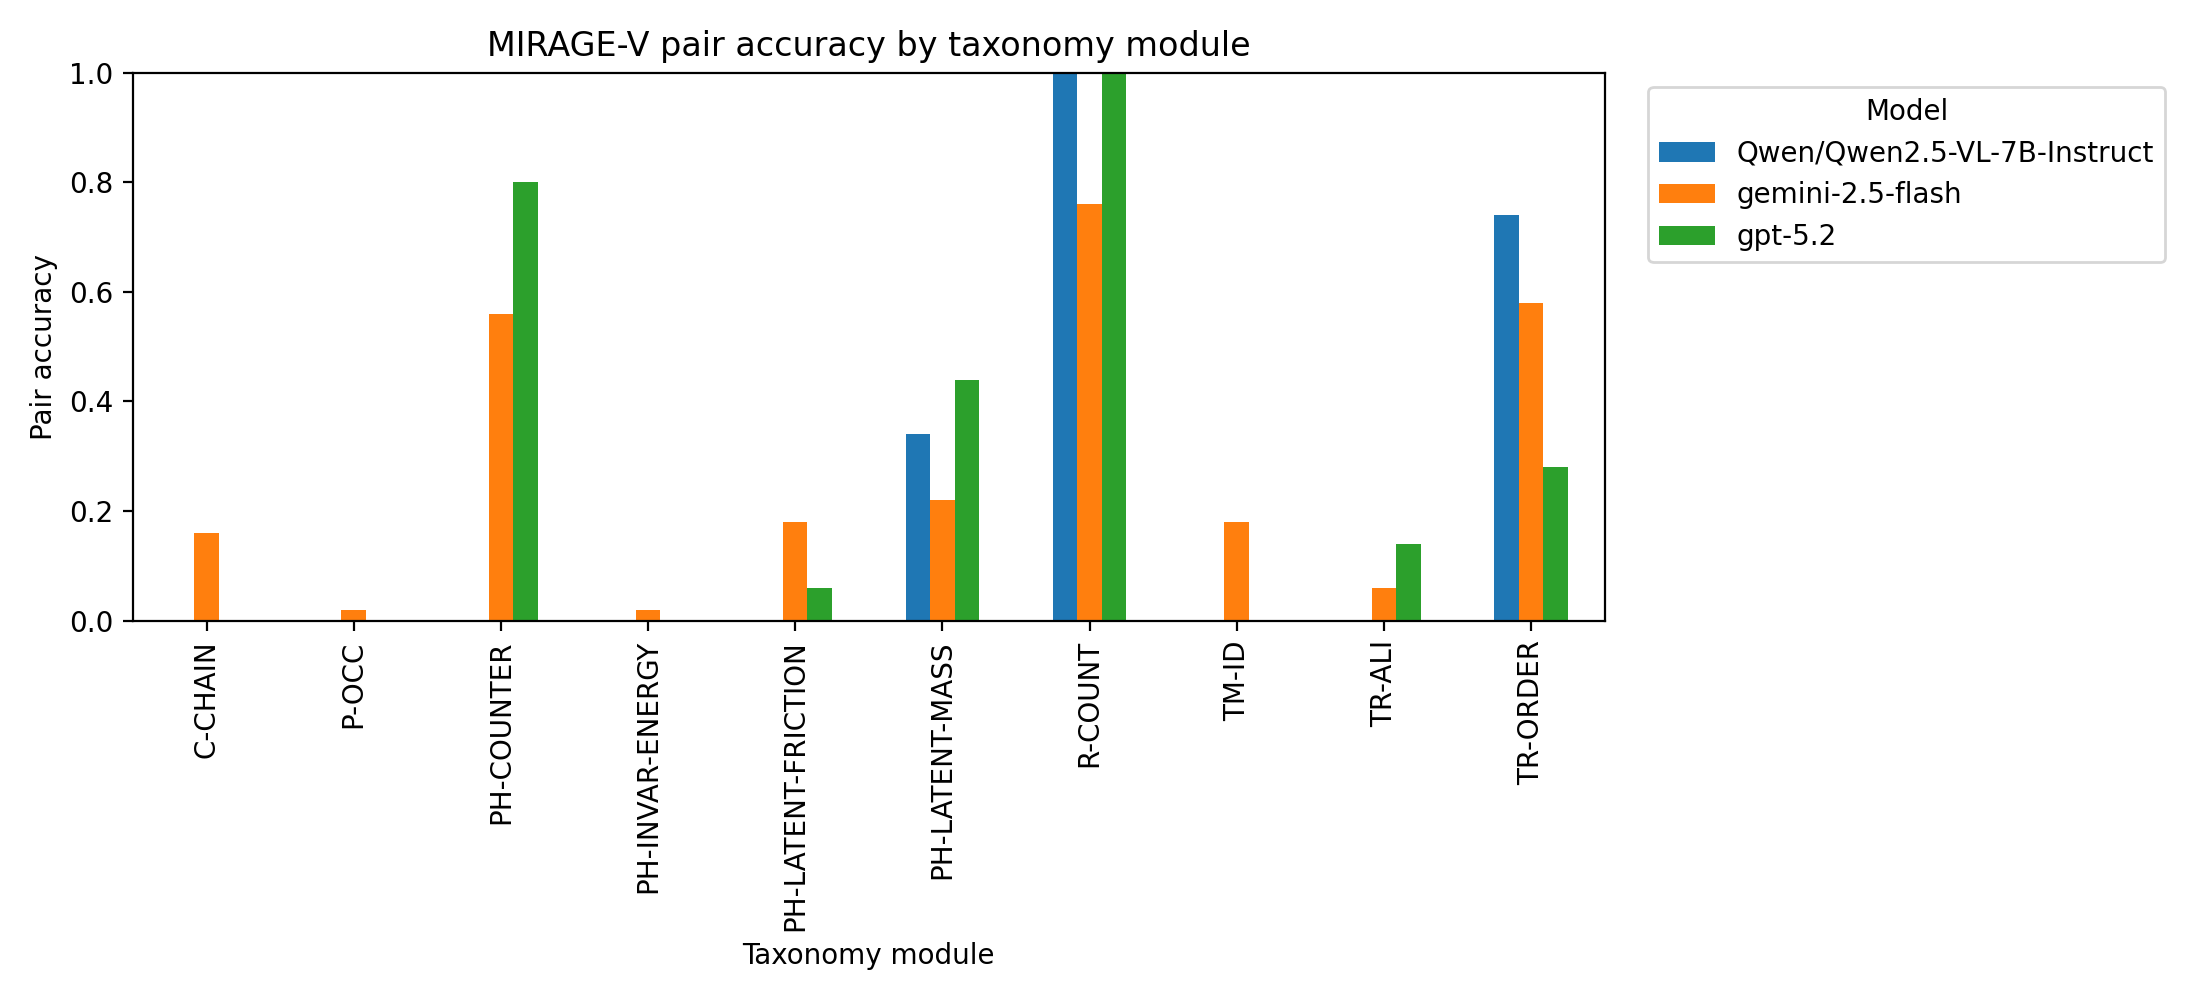
\includegraphics[width=\linewidth]{figures/pair_accuracy_by_module.png}
  \caption{Pair accuracy by taxonomy module. Pair accuracy measures whether a model can discriminate minimal-change pairs rather than relying on priors.}
  \label{fig:by-module-pair-accuracy}
\end{figure}

\begin{table}[t]
  \centering
  \small
  \caption{Per-module pair accuracy (\%, higher is better). Each module contains 50 minimal-change pairs.}
  \label{tab:by-module-pair-accuracy}
  % Auto-generated from pair_accuracy_by_module.csv
\begin{tabular}{lrrr}
\toprule
Module & Qwen2.5-VL-7B & Gemini-2.5-Flash & GPT-5.2 \\
\midrule
C-CHAIN & 0.0 & \textbf{16.0} & 0.0 \\
P-OCC & 0.0 & \textbf{2.0} & 0.0 \\
PH-COUNTER & 0.0 & 56.0 & \textbf{80.0} \\
PH-INVAR-ENERGY & 0.0 & \textbf{2.0} & 0.0 \\
PH-LATENT-FRICTION & 0.0 & \textbf{18.0} & 6.0 \\
PH-LATENT-MASS & 34.0 & 22.0 & \textbf{44.0} \\
R-COUNT & \textbf{100.0} & 76.0 & 100.0 \\
TM-ID & 0.0 & \textbf{18.0} & 0.0 \\
TR-ALI & 0.0 & 6.0 & \textbf{14.0} \\
TR-ORDER & \textbf{74.0} & 58.0 & 28.0 \\
\bottomrule
\end{tabular}
\end{table}

\subsection{Discussion}
Overall, the gap between accuracy and pair accuracy highlights a key evaluation pitfall: moderately high accuracy can arise from biased or shortcut answers, while pair accuracy directly tests whether the model's answer changes appropriately under minimal physical interventions.
MIRAGE-V makes these failure modes explicit through taxonomy labels, critical windows, and mandatory shortcut audits, enabling more actionable diagnosis than aggregate scores alone.

\section{Conclusion}
We introduced MIRAGE-V, a taxonomy-driven benchmark for physics checking in videos built from minimal-change paired clips with critical-window annotations.
Baseline results on three representative models show that while overall accuracy reaches at most \BestAcc\%, pair accuracy remains below \BestPairAcc\%, indicating that even strong models frequently fail to discriminate minimally different clips and to detect subtle physical inconsistencies.
Future work includes expanding coverage to more real-world edited videos, evaluating native-video interfaces under matched protocols, and developing training signals that explicitly optimize discrimination under minimal interventions.


\bibliographystyle{plain}
\bibliography{references}

\appendix
\section{Additional Details}
\subsection{Prompting and parsing}
All baseline runs use a constrained output format (``YES''/``NO'' only). 
We recommend using structured outputs where available to avoid empty or unparsable responses and to ensure consistent scoring across APIs.

\subsection{Reproducibility}
The released artifact includes:
(i) code to generate MIRAGE-V pairs, 
(ii) scripts to run evaluation across adapters (open-weight and API models), and 
(iii) utilities to aggregate runs into CSV tables and charts used in this paper.


\end{document}
